\chapter{Experiment s krátkou trasou a krátkym vozidlom}
\label{shortDshortV}

\begin{figure}[h]
  \centering
  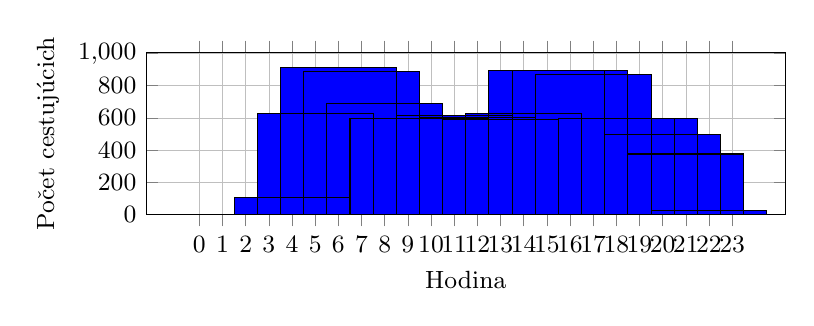
\begin{tikzpicture}
    \begin{axis}[
      width=0.8\textwidth,
      height=0.3\textwidth,
      xlabel={Hodina},
      ylabel={Počet cestujúcich},
      ymin=0,
      xtick={0,1,...,23},
      grid=both,
      major grid style={line width=.2pt,draw=gray!50},
      minor grid style={line width=.1pt,draw=gray!20},
      tick label style={font=\small},
      label style={font=\small},
      legend style={font=\small, at={(0.5,-0.2)}, anchor=north, legend columns=-1},
      ybar,
      bar width=5,
      ]
      \addplot[fill=blue] coordinates {
        (0, 0) (1, 0) (2, 0) (3, 0) (4, 104) (5, 625) (6, 915) (7, 888) 
        (8, 689) (9, 595) (10, 598) (11, 613) (12, 603) (13, 589) 
        (14, 630) (15, 894) (16, 897) (17, 872) (18, 597) (19, 597) 
        (20, 499) (21, 376) (22, 22) (23, 0)
      };
    \end{axis}
  \end{tikzpicture}
  \caption{Počet cestujúcich prichádzajúcich na zastávku za hodinu}
\end{figure}

\begin{figure}[h]
  \centering
  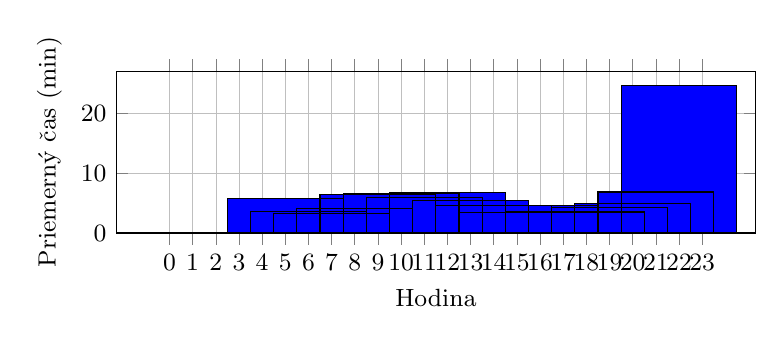
\begin{tikzpicture}
    \begin{axis}[
      width=0.8\textwidth,
      height=0.3\textwidth,
      xlabel={Hodina},
      ylabel={Priemerný čas (min)},
      ymin=0,
      xtick={0,1,...,23},
      grid=both,
      major grid style={line width=.2pt,draw=gray!50},
      minor grid style={line width=.1pt,draw=gray!20},
      tick label style={font=\small},
      label style={font=\small},
      legend style={font=\small, at={(0.5,-0.2)}, anchor=north, legend columns=-1},
      ybar,
      bar width=5,
      ]
      \addplot[fill=blue] coordinates {
        (0, 0) (1, 0) (2, 0) (3, 0) (4, 0) (5, 5.6816) (6, 3.5224043715846993) (7, 3.293918918918919) 
        (8, 4.0406386066763424) (9, 6.485714285714286) (10, 6.6003344481605355) (11, 5.993474714518761) 
        (12, 6.724709784411277) (13, 5.426146010186757) (14, 4.642857142857143) (15, 3.475391498881432) 
        (16, 4.517279821627648) (17, 3.5940366972477062) (18, 3.4974874371859297) (19, 4.239530988274707) 
        (20, 4.9318637274549095) (21, 6.843085106382978) (22, 24.545454545454547) (23, 0)
      };
    \end{axis}
  \end{tikzpicture}
  \caption{Priemerný čas strávený čakaním za hodinu}
\end{figure}

\begin{table}[h]
  \centering
  \begin{tabular}{|l|c|}
    \hline
    \textbf{Zastávka} & \# \\ \hline
    Lesná, Haškova & 0 \\ \hline
    Brechtova & 1 \\ \hline
    Blažkova & 2 \\ \hline
    Arbesova & 3 \\ \hline
    Heleny Malířové & 4 \\ \hline
    Lesná, nádraží & 5 \\ \hline
    Štefánikova čtvrť & 6 \\ \hline
    Provozníkova & 7 \\ \hline
    Lesnická & 9 \\ \hline
    Zemědělská & 10 \\ \hline
    Černá Pole, Erbenova & 11 \\ \hline
  \end{tabular}
  \caption{Rozpis zastávok}
\end{table}

\begin{table}[h]
  \centering
  \begin{tabular}{|c|l|}
    \hline
      \textbf{h} & \textbf{Odchody} \\ \hline
      05 & 00, 10, 20, 30, 40, 50 \\ \hline
      06 & 00, 06, 12, 18, 24, 30, 36, 42, 48, 54 \\ \hline
      07 & 00, 06, 13, 20, 26, 33, 40, 46, 53 \\ \hline
      08 & 00, 08, 17, 25, 34, 42, 51 \\ \hline
      09 & 00, 15, 30, 45 \\ \hline
      10 & 00, 12, 24, 36, 48 \\ \hline
      11 & 00, 12, 24, 36, 48 \\ \hline
      12 & 00, 15, 30, 45 \\ \hline
      13 & 00, 08, 17, 25, 34, 42, 51 \\ \hline
      14 & 00, 10, 20, 30, 40, 50 \\ \hline
      15 & 00, 06, 12, 18, 24, 30, 36, 42, 48, 54 \\ \hline
      16 & 00, 10, 20, 30, 40, 50 \\ \hline
      17 & 00, 06, 12, 18, 24, 30, 36, 42, 48, 54 \\ \hline
      18 & 00, 07, 15, 22, 30, 37, 45, 52 \\ \hline
      19 & 00, 08, 17, 25, 34, 42, 51 \\ \hline
      20 & 00, 10, 20, 30, 40, 50 \\ \hline
      21 & 00, 15, 30, 45 \\ \hline
      22 & 00 \\ \hline
  \end{tabular}
  \caption{Časový rozpis}
\end{table}
